\subsection{Support Vector Machine}

\begin{figure}[h]
\center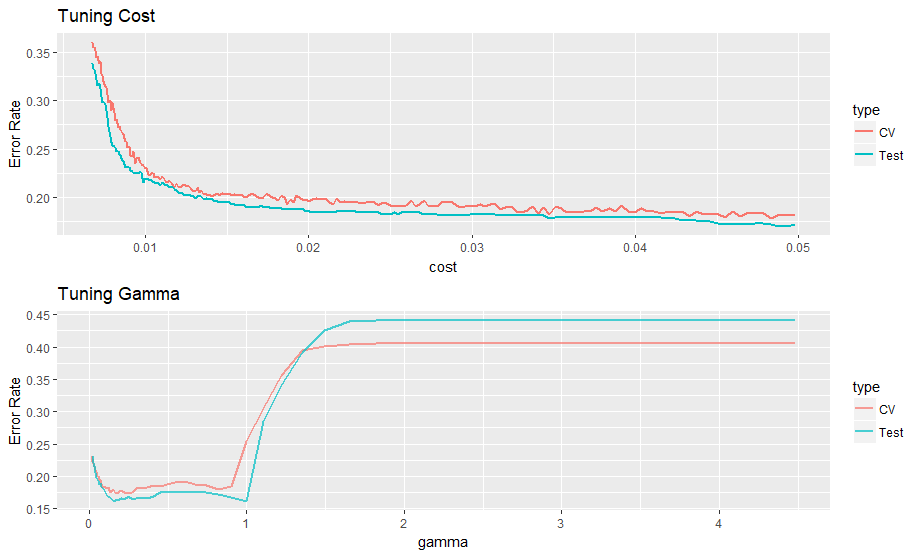
\includegraphics[width = .8\textwidth]{svm.png}
\caption{Parameter Tuning of SVM}
\label{svm}
\end{figure}

Kernel support vector machines (SVMs) are supervised learning models with associated learning algorithms commonly used in classification.\cite{cristianini2000introduction}

The effectiveness of SVM depends on the selection of kernel, the kernel's parameters, and soft margin parameter C. A common choice is a Gaussian kernel, which has a single parameter $\gamma$. The best combination of C and $\gamma$ is often selected by a grid search with exponentially growing sequences of C and $\gamma$. Each combination of parameter choices is checked using cross validation, and the parameters with best cross-validation accuracy are picked. We can do this with function \emph{tune} given a list of C. In Figure \ref{svm} we can see the CV error and test error of SVM using different cost and gamma. The best C is 0.05 and the best $\gamma$ is 0.135.

With the parameters tunned we can conduct classfication. The test error are shown in Table \ref{tblsvm}. The Type \uppercase\expandafter{\romannumeral1} error is slightly larger than random forest, but Type \uppercase\expandafter{\romannumeral2} error is significantly lower than random forest. So SVM made less mistake in predicting raining days compared to random forest. This could partly be explained by the fact that this isn't a linearly separable case. 

\begin{table}[h]
\setlength{\belowcaptionskip}{5pt}
\caption{Confusion Matrix and Error Rates of SVM}
\label{tblsvm}
\centering
\renewcommand\arraystretch{1.5}
\begin{tabular}{rrrrr}
\hline
\hline
 & & \multicolumn{2}{c}{True Condition} & \\
\hline
 & & Non-Precipitation & Precipitation & \\
\cline{1-4}
\multirow{2}{*}{Prediction} & {Non-Precipitation} & 326 & 47 & \\
\cline{2-4}
&Precipitation&54&231&\\
\hline
&Error Rate & 0.142 & 0.169 & 0.1535\\
\cline{2-5}
& & Type \uppercase\expandafter{\romannumeral1} & Type \uppercase\expandafter{\romannumeral2} & Overall\\
\hline
\end{tabular}
\end{table}